
\section{Benchmarking msMINRES-CIQ}
\label{sec:ciq_empirical}

In this section we empirically measure the convergence and speedup of msMINRES-CIQ applied to several types of covariance matrices.

\paragraph{Convergence of CIQ.}
In \cref{fig:quad_error} we measure the relative error of computing $\bK^{1/2} \bb$ with msMINRES-CIQ on random matrices.\footnote{
	msMINRES is stopped after achieving a relative residual of $10^{-4}$ or after reaching $J=400$ iterations.
}
We vary
%
\begin{enumerate*}
  \item the number of quadrature points $Q$;
  \item the size of the matrix $N$; and
  \item the conditioning of the matrix.
\end{enumerate*}
%
The figure displays results for matrices with spectra that decay as $\lambda_t = 1 / \sqrt{t}$, $\lambda_t = 1/t$, $\lambda_t = 1 / t^2$, and $\lambda_t = e^{-t}$,
as well as for one-dimensional RBF and Mat\'ern kernel matrices (formed with random data), which have near-exponentially decaying spectra.
Consequently, the $1 / \sqrt{t}$ matrices are relatively well-conditioned, while the RBF/Mat\'ern kernels are relatively ill-conditioned.
Nevertheless, in all cases msMINRES-CIQ achieves $10^{-4}$ relative error with only $Q=8$ quadrature points, regardless of the size of the matrix.
Approximation algorithms like randomized SVD on the other hand incur an order of magnitude more error (\cref{fig:randomized_svd_supp}); a rank of $R=1,\!024$ is unable to reduce the relative error to a single decimal point.

\begin{figure}[t!]
	\centering
	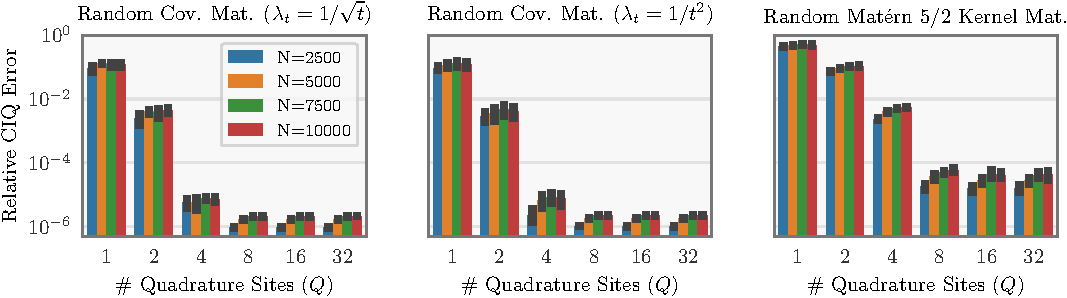
\includegraphics[width=\textwidth]{figures/quad_error.pdf}

	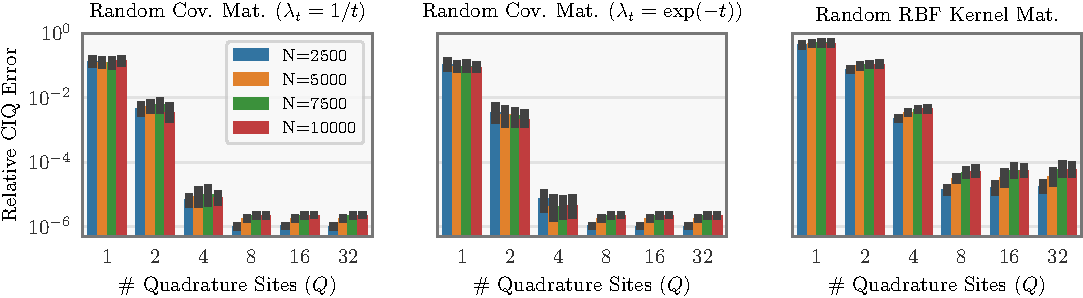
\includegraphics[width=\textwidth]{figures/quad_error_supp.pdf}
  \caption[
    Relative error of msMINRES-CIQ as a function of number of quadrature points $Q$.
  ]{
    msMINRES-CIQ relative error at computing $\bK^{1/2} \bb$ as a function of number of quadrature points $Q$.
    We test random matrices with eigenvalues that scale as $\lambda_t = 1/\sqrt{t}$ (top left), $\lambda_t = 1/t$ (bottom left), $\lambda_t = 1/{t}^2$ (top middle), and $\lambda_t = e^{-t}$ (bottom middle).
    Additionally, we test random Mat\'ern/RBF kernel matrices (top right/bottom right).
    In all cases $Q=8$ achieves $<10^{-4}$ error.
  }
  \label{fig:quad_error}
\end{figure}

\begin{figure}[ht!]
	\centering
	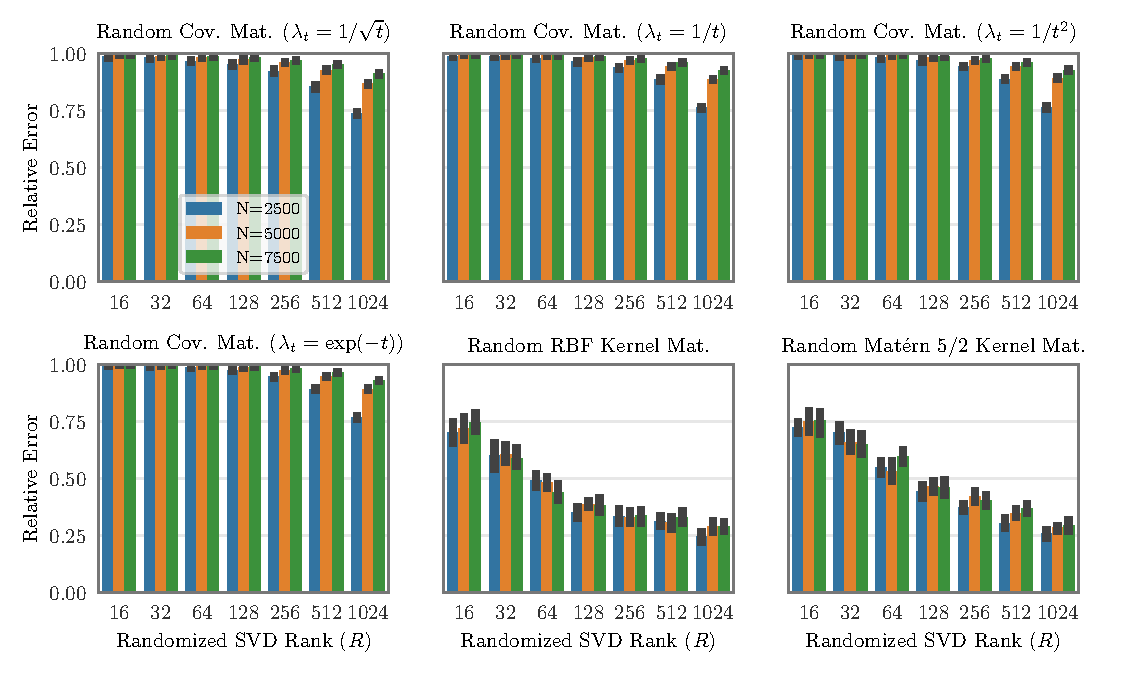
\includegraphics[width=\textwidth]{figures/randomized_svd_error_supp.pdf}
  \caption[
    Relative error of randomized SVD as a function of rank $R$.
  ]{
    Randomized SVD relative error at computing $\bK^{1/2} \bb$ as a function of approximation rank $R$.
    In all cases, randomized SVD is unable to achieve a relative error better than about $0.25$.
  }
  \label{fig:randomized_svd_supp}
\end{figure}

\begin{figure}[ht!]
	\centering
	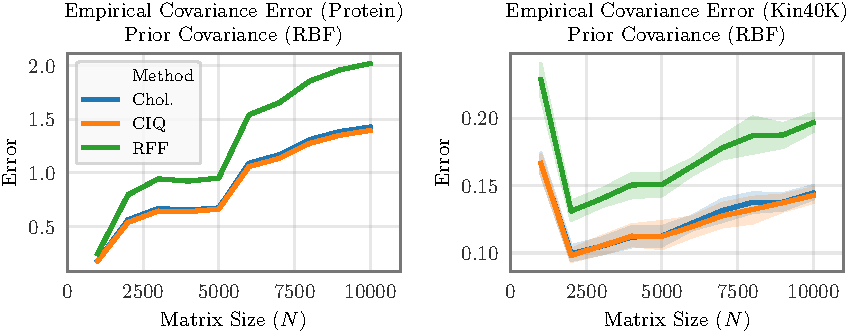
\includegraphics[width=0.85\textwidth]{figures/empirical_covariance_prior.pdf}
  \caption[
    Empirical covariance error of various sampling methods (Cholesky, msMINRES-CIQ, and Random Fourier Features).
  ]{
    Empirical covariance error (relative norm) of various sampling methods (Cholesky, msMINRES-CIQ, and $1,\!000$ Random Fourier Features \cite{rahimi2008random}).
    Empirical covariances are measured from $1,\!000$ samples.
    RBF matrices are constructed from data in the Protein and Kin40k datasets \cite{asuncion2007uci}.
  }
  \label{fig:empirical_covariance_matrix}
\end{figure}

To further compare msMINRES-CIQ to randomized methods, \cref{fig:empirical_covariance_matrix} plots the empirical covariance matrix of $1,\!000$ Gaussian samples drawn from a Gaussian process prior $\normaldist{\bzero}{\bK}$.
We construct the RBF covariance matrices $\bK$ using subsets of the Protein and Kin40k datasets \cite{asuncion2007uci}.
We note that all methods incur some sampling error, regardless of the subset size ($N$).
msMINRES-CIQ and Cholesky-based sampling tend to have very similar empirical covariance error.
On the other hand, the Random Fourier Features method \cite{rahimi2008random} (with $1,\!000$ random features) incurs errors up to $2\times$ as large.
This additional error is due to the randomness in the RFF approximation.

\begin{figure}[t!]
	\centering
	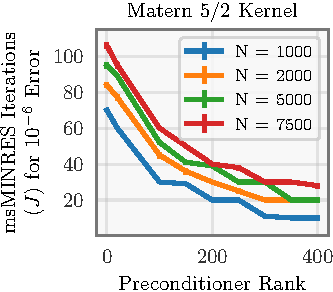
\includegraphics[width=0.4\textwidth]{figures/precond_result.pdf}
  \quad
	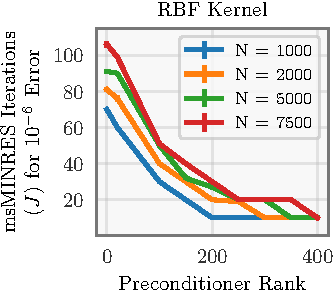
\includegraphics[width=0.4\textwidth]{figures/precond_result_rbf.pdf}
  \caption[
    Effect of preconditioning msMINRES-CIQ.
  ]{
    Effect of preconditioning msMINRES-CIQ (random Mat\'ern and RBF kernels with a pivoted Cholesky preconditioner).
    Larger preconditioners reduce the number of msMINRES iterations required to reach $10^{-6}$ error.
  }
  \label{fig:precond_result}
\end{figure}

Typically $J=100$ msMINRES iterations suffices for convergence; however this number can be lowered with preconditioning.
To demonstrate this, we construct  random $N \times N$ Mat\'ern/RBF kernels $\bK$, applying CIQ to a set of $N$ orthonormal vectors ($[\bK^{1/2} \bb_{1}, \ldots, \bK^{1/2} \bb_{N}]$), and compute the empirical covariance.
In \cref{fig:precond_result} we plot the number of msMINRES iterations needed to achieve a relative error of $10^{-6}$.
The pivoted Cholesky preconditioner of \cref{sec:preconditioning}---which forms a low-rank approximation of $\bK$---accelerates convergence of msMINRES.
Without preconditioning (i.e. rank=0), $J=100$ iterations are required for $N=7,\!500$ matrices.
With rank-100/rank-400 preconditioners, iterations are cut by a factor of two/four.

\begin{figure}[t!]
	\centering
	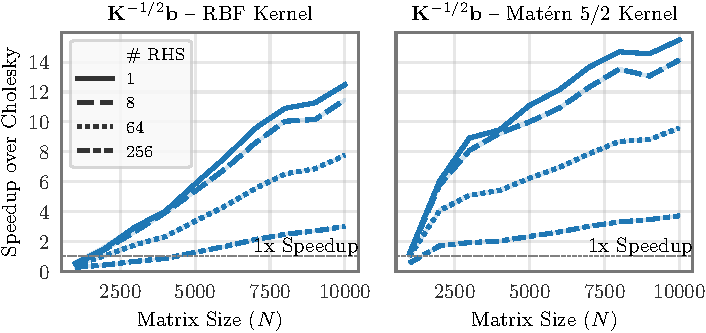
\includegraphics[width=0.8\textwidth]{figures/timing.pdf}
  \caption[
    Speedup of msMINRES-CIQ over Cholesky.
  ]{
    Speedup of msMINRES-CIQ over Cholesky when computing forward/backward passes of $\bK^{-\frac 1 2} \bb$ w/ varying number of right-hand-sides (RHS).
  }
  \label{fig:timing}
\end{figure}

\paragraph{Speedup over Cholesky.}
We compare the wall-clock speedup of msMINRES-CIQ over Cholesky in \cref{fig:timing} on RBF/Mat\'ern kernels.\footnote{
  $Q=8$.
  msMINRES is stopped after a residual of $10^{-4}$.
  Kernels are formed using data from the Kin40k dataset \citep{asuncion2007uci}.
  Timings are performed on a NVIDIA 1070 GPU.
}
We compute $\bK^{-1/2} \bb$ and its derivative on multiple right-hand-side (RHS) vectors.
As $N$ increases, msMINRES-CIQ incurs a larger speedup (up to $15\times$ faster than Cholesky).
This speedup is less pronounced when computing many RHSs simultaneously, as the cubic complexity of Cholesky is amortized across each RHS.
Nevertheless, msMINRES-CIQ is advantageous for matrices larger than $N=3,\!000$ even when simultaneously whitening $256$ vectors.
